
\begin{frame}\frametitle{Test Image} 
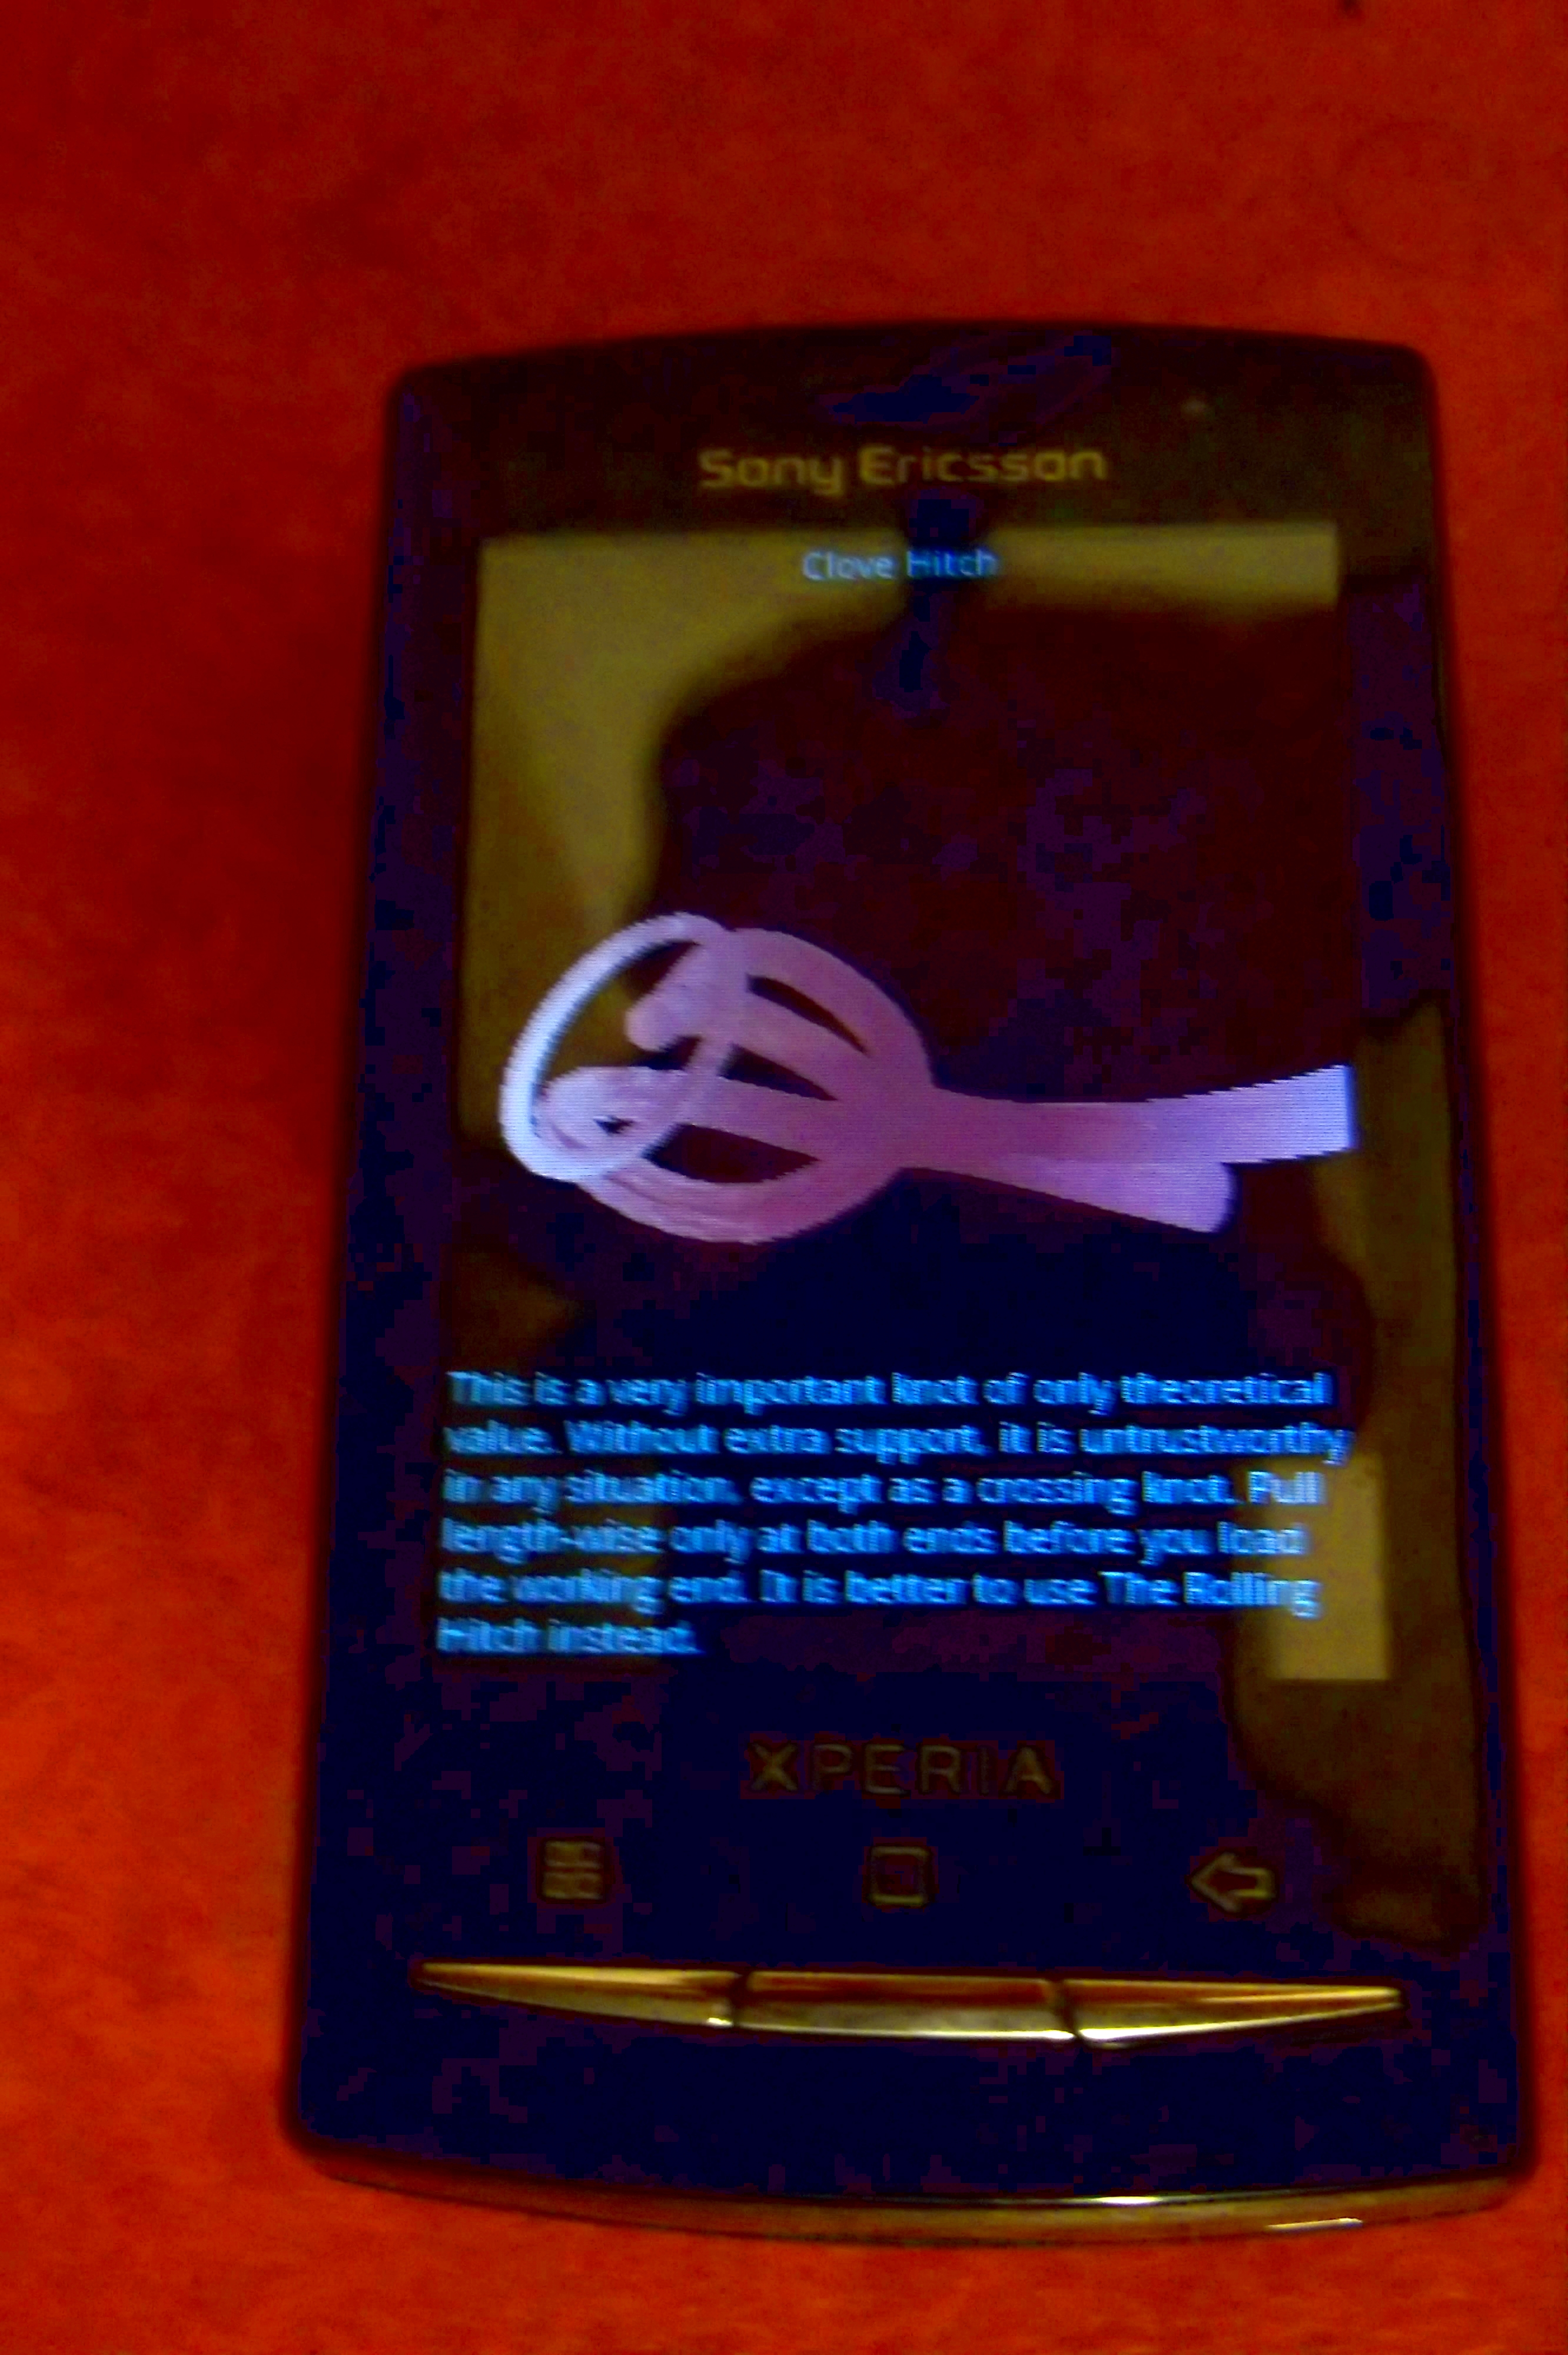
\includegraphics[height=8cm]{clove_hitch1.jpg}
\end{frame}

\begin{frame}\frametitle{Test Image} 
\includegraphics[height=8cm]{clove_hitch2.jpg}
\end{frame}

\begin{frame} \frametitle{INE Skyline (SK)} 
  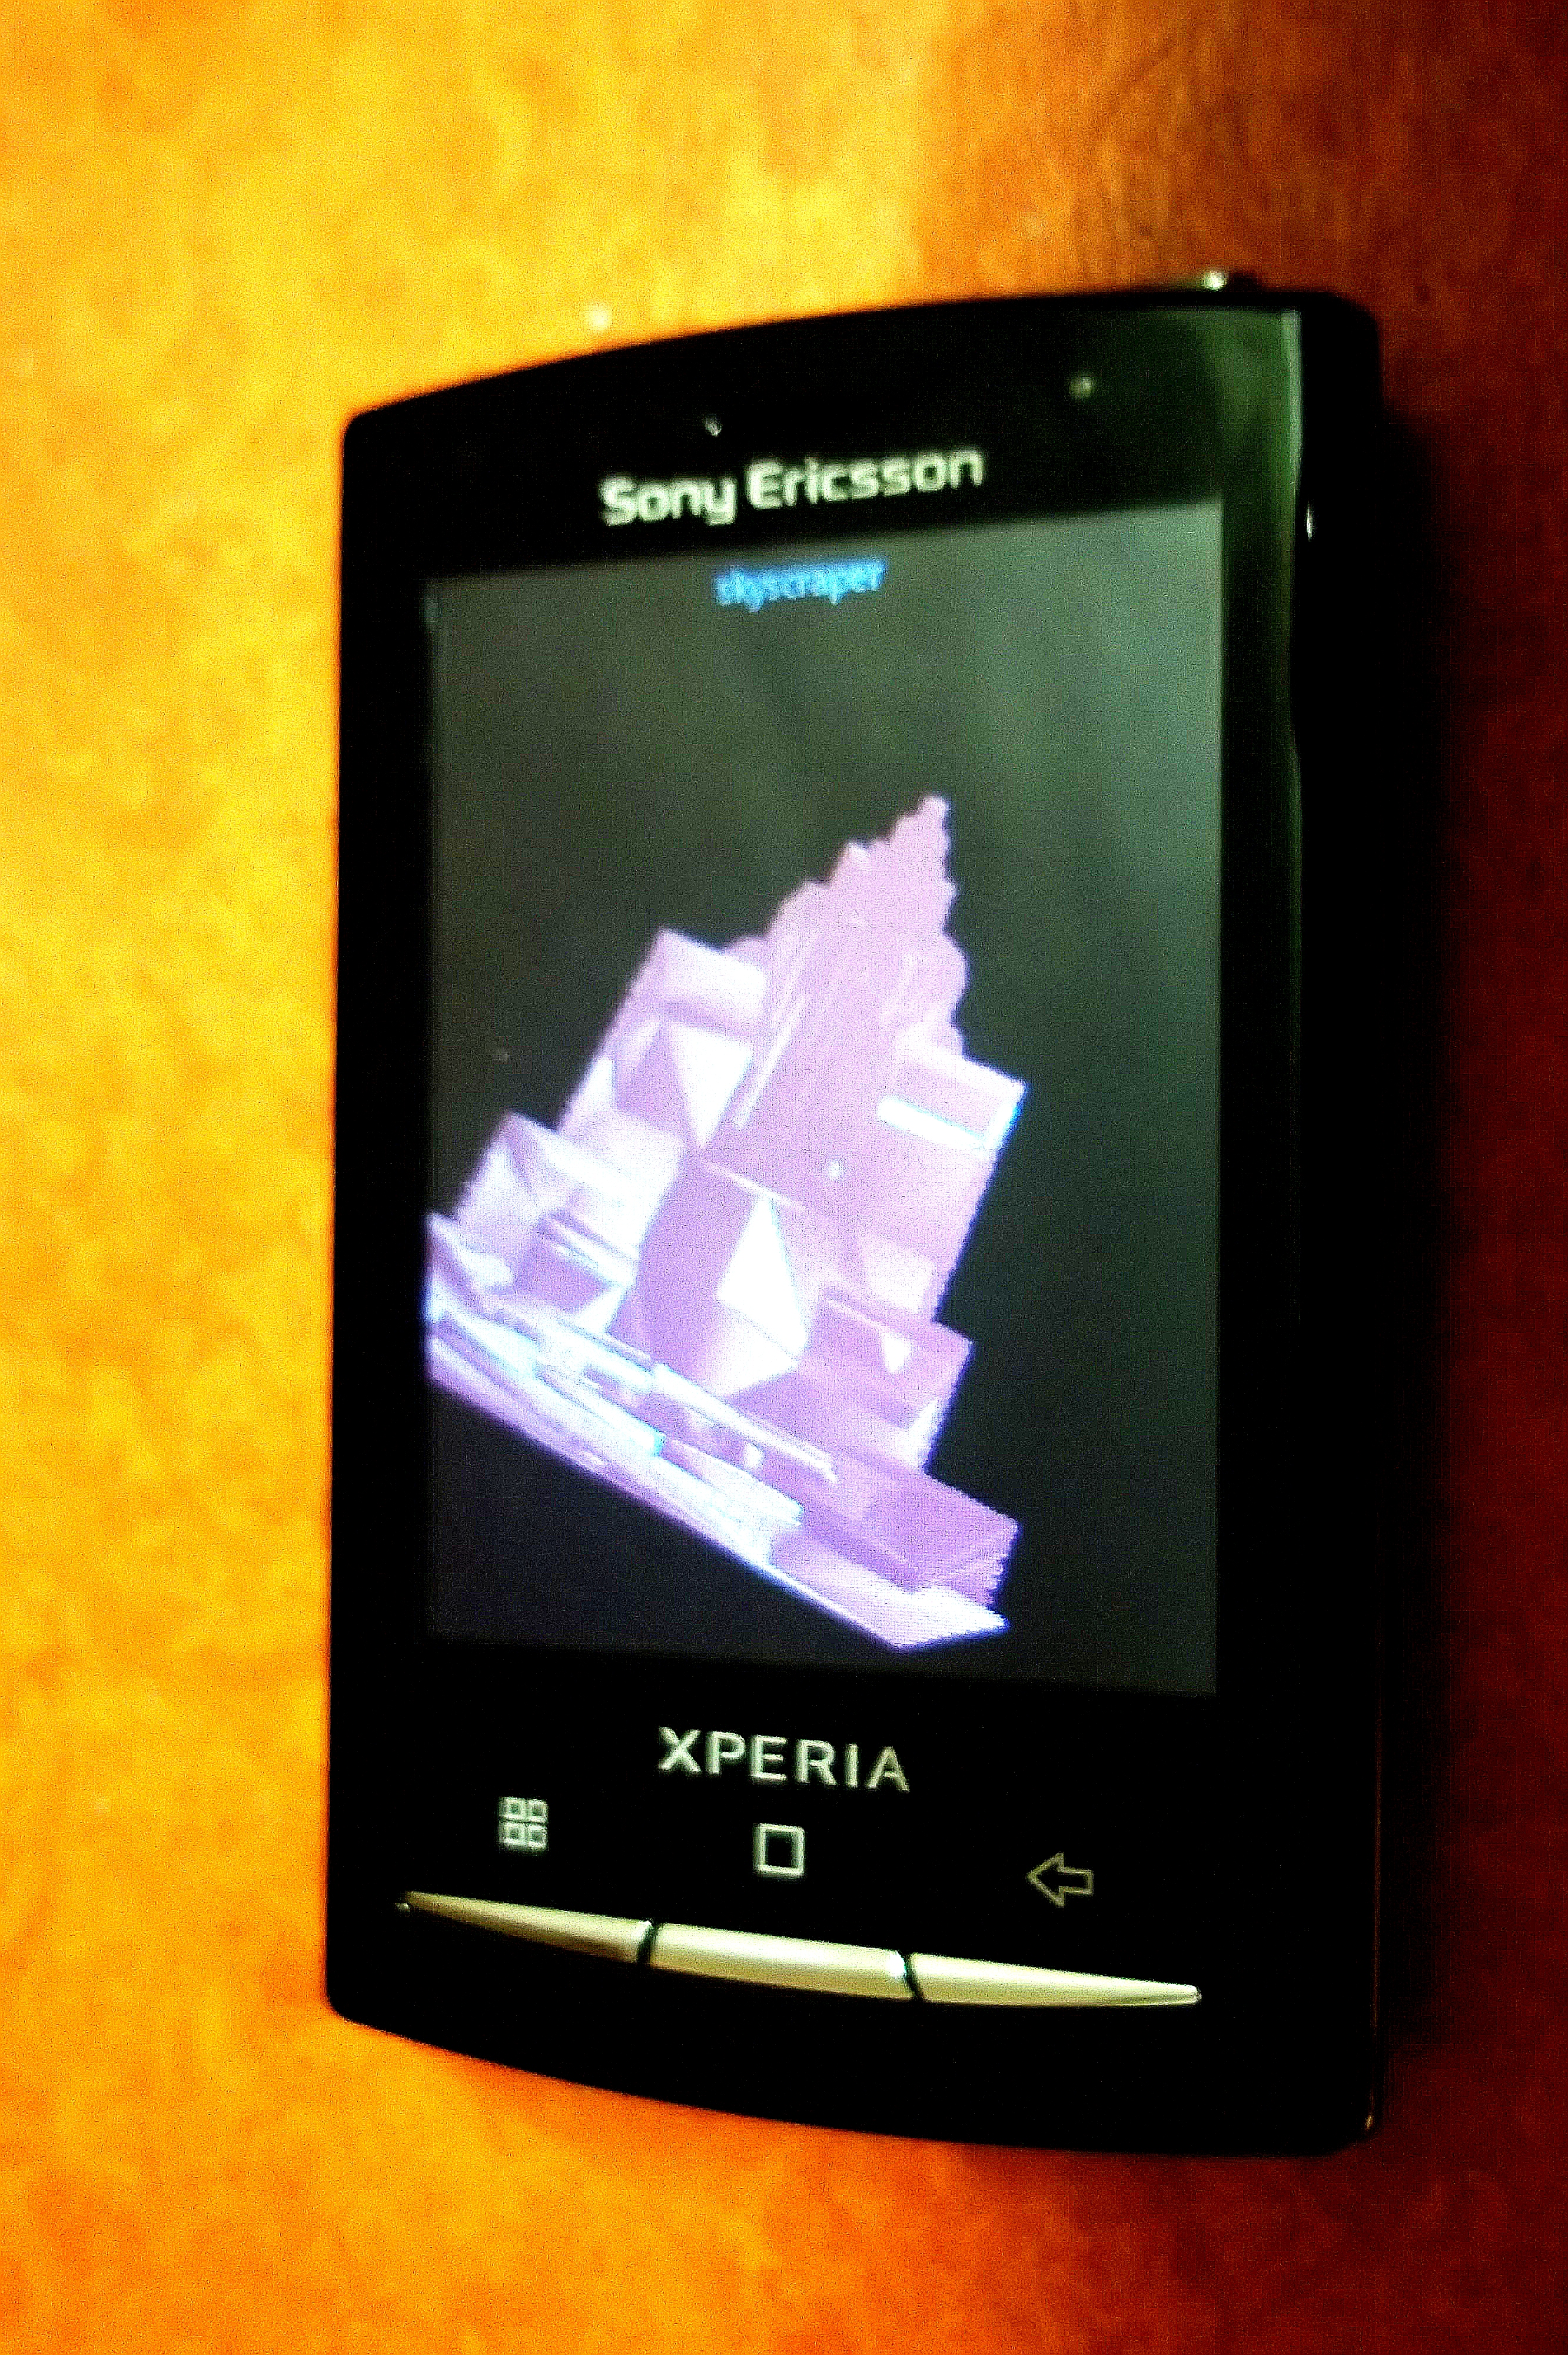
\includegraphics[height=8cm]{skyscraper.jpg}
\end{frame}

\begin{frame}\frametitle{Test Image} 
\includegraphics[height=8cm]{structure.png}
\end{frame}

\begin{frame}\frametitle{Test Image} 
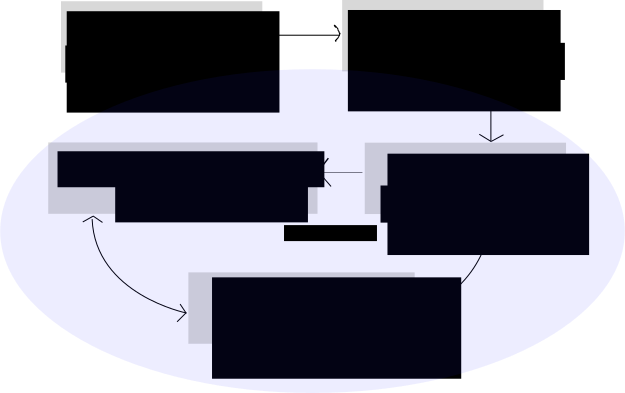
\includegraphics[height=8cm]{work_flow.png}
\end{frame}

\begin{frame}\frametitle{Test Image} 
\includegraphics[height=8cm]{x11renderer.png}
\end{frame}

\begin{frame}\frametitle{Test Image} 
\includegraphics[height=8cm]{sdcard.png}
\end{frame}

\begin{frame}\frametitle{Time estimation} 
\begin{tabular}{| l || c | c |  c | c |}
\hline
Feature & Priority & Implemented & Est. hours & Real hours\\
\hline
\hline
\textbf{Learning JNI} & high & YES &                 4 & 51.5\\
\textbf{Exploring ndk samples} & high & YES &       12 & 11.5\\
\textbf{OpenGL demo} & high & YES &                  4 & 25\\
\textbf{Running animation} & high & YES &           20 & 40\\
\textbf{Loading OBJ definition} & high & YES &       6 &  8.5\\
\textbf{Select model} & high & YES &                 1 & 10\\
\textbf{Full screen} & middle & YES &                3 &  0\\
\textbf{Screen saver} & middle & NO &                4 &  -\\
\textbf{Binding colourising} & middle & NO &         4 & -\\
\textbf{Viewpoint manual} change & low & YES &       2 & 5\\
\textbf{Docs \& refactoring} & middle & NO &         5 & 20\\
\textbf{Design of XML} & high & NO &                15 & 1\\
\hline
\textbf{Totally} & &                                80 & 172.5 \\
\hline
\end{tabular}

\end{frame}

